\documentclass[1p]{elsarticle_modified}
%\bibliographystyle{elsarticle-num}

%\usepackage[colorlinks]{hyperref}
%\usepackage{abbrmath_seonhwa} %\Abb, \Ascr, \Acal ,\Abf, \Afrak
\usepackage{amsfonts}
\usepackage{amssymb}
\usepackage{amsmath}
\usepackage{amsthm}
\usepackage{scalefnt}
\usepackage{amsbsy}
\usepackage{kotex}
\usepackage{caption}
\usepackage{subfig}
\usepackage{color}
\usepackage{graphicx}
\usepackage{xcolor} %% white, black, red, green, blue, cyan, magenta, yellow
\usepackage{float}
\usepackage{setspace}
\usepackage{hyperref}

\usepackage{tikz}
\usetikzlibrary{arrows}

\usepackage{multirow}
\usepackage{array} % fixed length table
\usepackage{hhline}

%%%%%%%%%%%%%%%%%%%%%
\makeatletter
\renewcommand*\env@matrix[1][\arraystretch]{%
	\edef\arraystretch{#1}%
	\hskip -\arraycolsep
	\let\@ifnextchar\new@ifnextchar
	\array{*\c@MaxMatrixCols c}}
\makeatother %https://tex.stackexchange.com/questions/14071/how-can-i-increase-the-line-spacing-in-a-matrix
%%%%%%%%%%%%%%%

\usepackage[normalem]{ulem}

\newcommand{\msout}[1]{\ifmmode\text{\sout{\ensuremath{#1}}}\else\sout{#1}\fi}
%SOURCE: \msout is \stkout macro in https://tex.stackexchange.com/questions/20609/strikeout-in-math-mode

\newcommand{\cancel}[1]{
	\ifmmode
	{\color{red}\msout{#1}}
	\else
	{\color{red}\sout{#1}}
	\fi
}

\newcommand{\add}[1]{
	{\color{blue}\uwave{#1}}
}

\newcommand{\replace}[2]{
	\ifmmode
	{\color{red}\msout{#1}}{\color{blue}\uwave{#2}}
	\else
	{\color{red}\sout{#1}}{\color{blue}\uwave{#2}}
	\fi
}

\newcommand{\Sol}{\mathcal{S}} %segment
\newcommand{\D}{D} %diagram
\newcommand{\A}{\mathcal{A}} %arc


%%%%%%%%%%%%%%%%%%%%%%%%%%%%%5 test

\def\sl{\operatorname{\textup{SL}}(2,\Cbb)}
\def\psl{\operatorname{\textup{PSL}}(2,\Cbb)}
\def\quan{\mkern 1mu \triangleright \mkern 1mu}

\theoremstyle{definition}
\newtheorem{thm}{Theorem}[section]
\newtheorem{prop}[thm]{Proposition}
\newtheorem{lem}[thm]{Lemma}
\newtheorem{ques}[thm]{Question}
\newtheorem{cor}[thm]{Corollary}
\newtheorem{defn}[thm]{Definition}
\newtheorem{exam}[thm]{Example}
\newtheorem{rmk}[thm]{Remark}
\newtheorem{alg}[thm]{Algorithm}

\newcommand{\I}{\sqrt{-1}}
\begin{document}

%\begin{frontmatter}
%
%\title{Boundary parabolic representations of knots up to 8 crossings}
%
%%% Group authors per affiliation:
%\author{Yunhi Cho} 
%\address{Department of Mathematics, University of Seoul, Seoul, Korea}
%\ead{yhcho@uos.ac.kr}
%
%
%\author{Seonhwa Kim} %\fnref{s_kim}}
%\address{Center for Geometry and Physics, Institute for Basic Science, Pohang, 37673, Korea}
%\ead{ryeona17@ibs.re.kr}
%
%\author{Hyuk Kim}
%\address{Department of Mathematical Sciences, Seoul National University, Seoul 08826, Korea}
%\ead{hyukkim@snu.ac.kr}
%
%\author{Seokbeom Yoon}
%\address{Department of Mathematical Sciences, Seoul National University, Seoul, 08826,  Korea}
%\ead{sbyoon15@snu.ac.kr}
%
%\begin{abstract}
%We find all boundary parabolic representation of knots up to 8 crossings.
%
%\end{abstract}
%\begin{keyword}
%    \MSC[2010] 57M25 
%\end{keyword}
%
%\end{frontmatter}

%\linenumbers
%\tableofcontents
%
\newcommand\colored[1]{\textcolor{white}{\rule[-0.35ex]{0.8em}{1.4ex}}\kern-0.8em\color{red} #1}%
%\newcommand\colored[1]{\textcolor{white}{ #1}\kern-2.17ex	\textcolor{white}{ #1}\kern-1.81ex	\textcolor{white}{ #1}\kern-2.15ex\color{red}#1	}

{\Large $\underline{12n_{0808}~(K12n_{0808})}$}

\setlength{\tabcolsep}{10pt}
\renewcommand{\arraystretch}{1.6}
\vspace{1cm}\begin{tabular}{m{100pt}>{\centering\arraybackslash}m{274pt}}
\multirow{5}{120pt}{
	\centering
	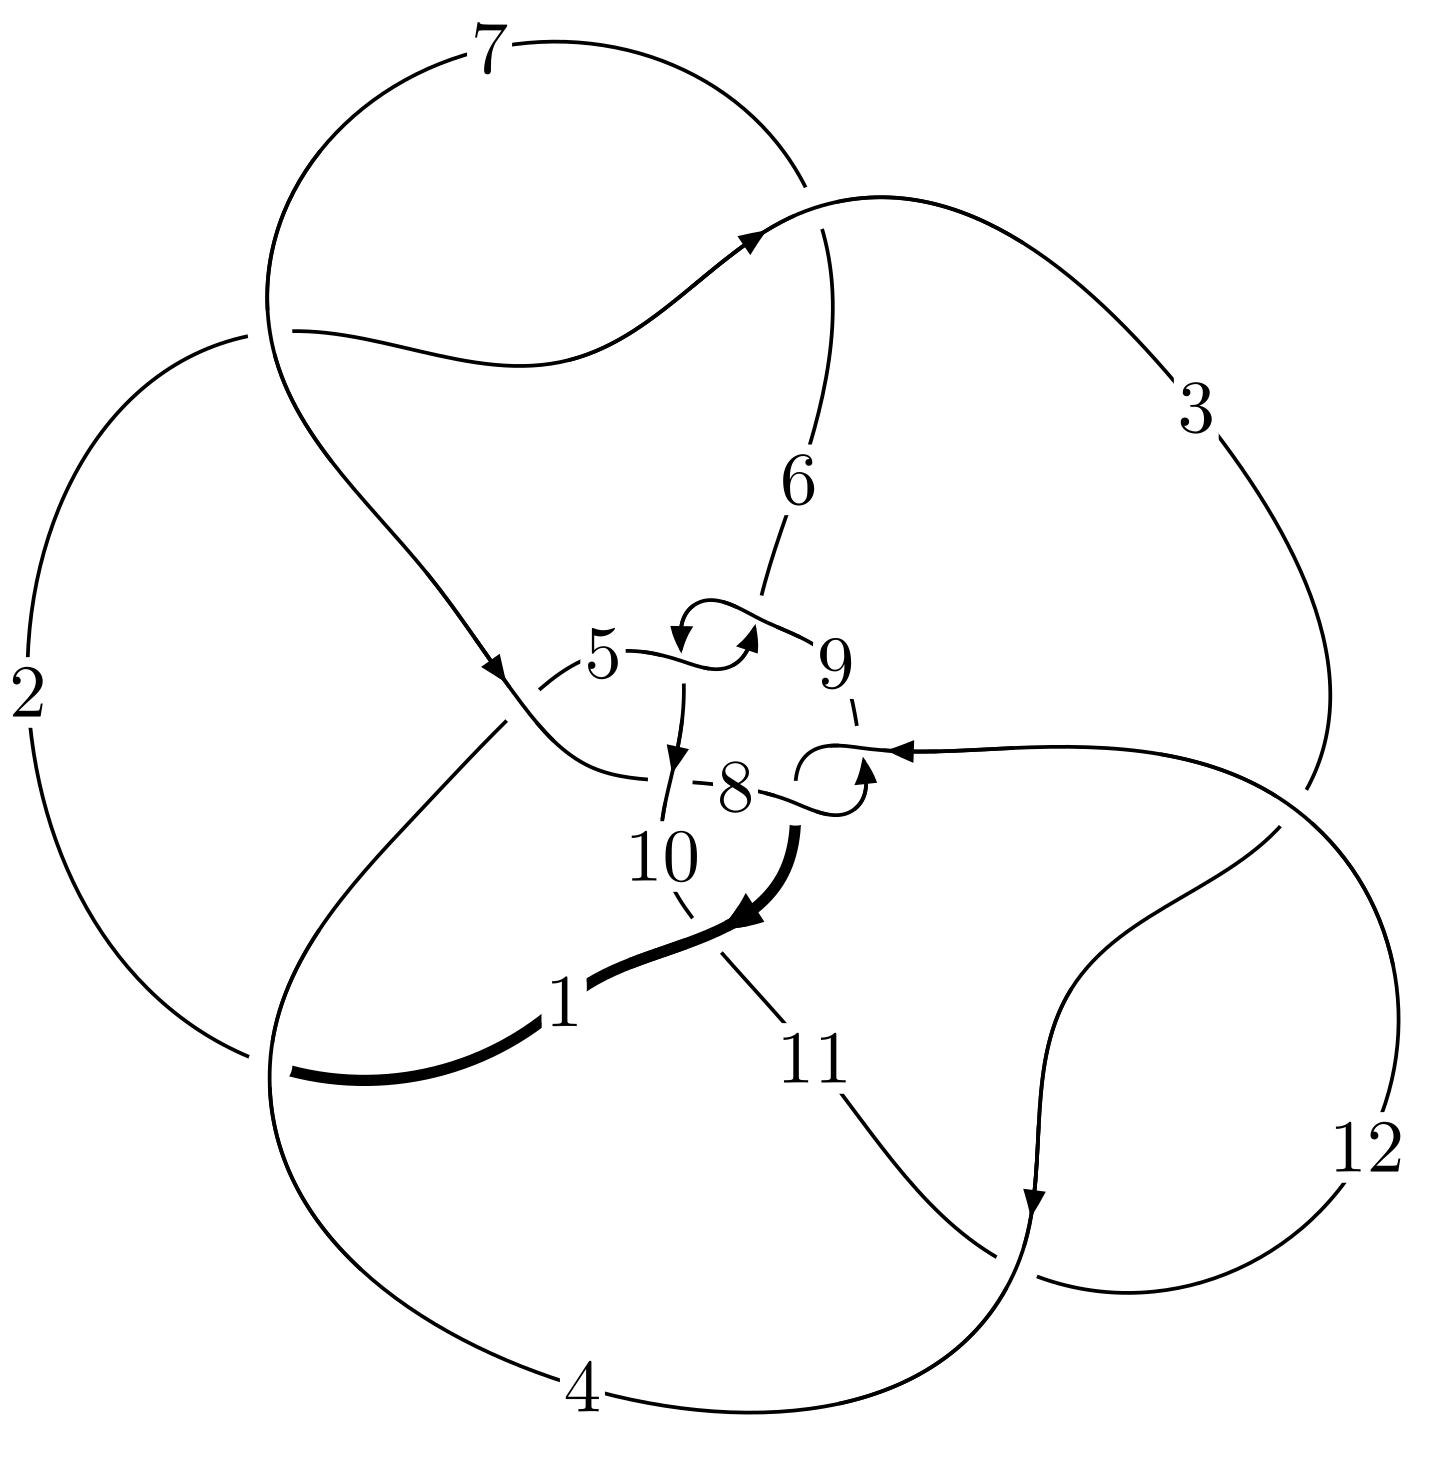
\includegraphics[width=112pt]{../../../GIT/diagram.site/Diagrams/png/2897_12n_0808.png}\\
\ \ \ A knot diagram\footnotemark}&
\allowdisplaybreaks
\textbf{Linearized knot diagam} \\
\cline{2-2}
 &
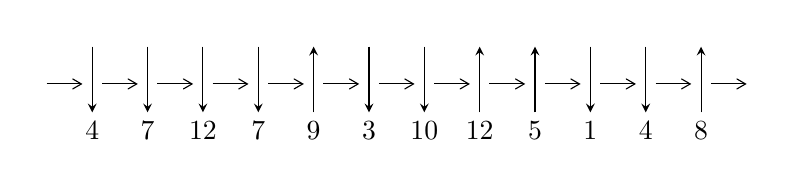
\begin{tikzpicture}[x=20pt, y=17pt]
	% nodes
	\node (C0) at (0, 0) {};
	\node (C1) at (1, 0) {};
	\node (C1U) at (1, +1) {};
	\node (C1D) at (1, -1) {4};

	\node (C2) at (2, 0) {};
	\node (C2U) at (2, +1) {};
	\node (C2D) at (2, -1) {7};

	\node (C3) at (3, 0) {};
	\node (C3U) at (3, +1) {};
	\node (C3D) at (3, -1) {12};

	\node (C4) at (4, 0) {};
	\node (C4U) at (4, +1) {};
	\node (C4D) at (4, -1) {7};

	\node (C5) at (5, 0) {};
	\node (C5U) at (5, +1) {};
	\node (C5D) at (5, -1) {9};

	\node (C6) at (6, 0) {};
	\node (C6U) at (6, +1) {};
	\node (C6D) at (6, -1) {3};

	\node (C7) at (7, 0) {};
	\node (C7U) at (7, +1) {};
	\node (C7D) at (7, -1) {10};

	\node (C8) at (8, 0) {};
	\node (C8U) at (8, +1) {};
	\node (C8D) at (8, -1) {12};

	\node (C9) at (9, 0) {};
	\node (C9U) at (9, +1) {};
	\node (C9D) at (9, -1) {5};

	\node (C10) at (10, 0) {};
	\node (C10U) at (10, +1) {};
	\node (C10D) at (10, -1) {1};

	\node (C11) at (11, 0) {};
	\node (C11U) at (11, +1) {};
	\node (C11D) at (11, -1) {4};

	\node (C12) at (12, 0) {};
	\node (C12U) at (12, +1) {};
	\node (C12D) at (12, -1) {8};
	\node (C13) at (13, 0) {};

	% arrows
	\draw[->,>={angle 60}]
	(C0) edge (C1) (C1) edge (C2) (C2) edge (C3) (C3) edge (C4) (C4) edge (C5) (C5) edge (C6) (C6) edge (C7) (C7) edge (C8) (C8) edge (C9) (C9) edge (C10) (C10) edge (C11) (C11) edge (C12) (C12) edge (C13) ;	\draw[->,>=stealth]
	(C1U) edge (C1D) (C2U) edge (C2D) (C3U) edge (C3D) (C4U) edge (C4D) (C5D) edge (C5U) (C6U) edge (C6D) (C7U) edge (C7D) (C8D) edge (C8U) (C9D) edge (C9U) (C10U) edge (C10D) (C11U) edge (C11D) (C12D) edge (C12U) ;
	\end{tikzpicture} \\
\hhline{~~} \\& 
\textbf{Solving Sequence} \\ \cline{2-2} 
 &
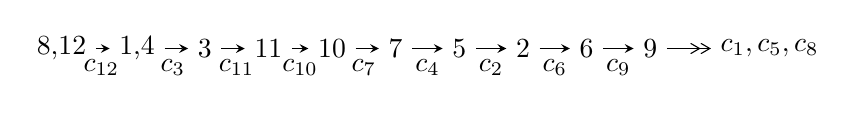
\begin{tikzpicture}[x=23pt, y=7pt]
	% node
	\node (A0) at (-1/8, 0) {8,12};
	\node (A1) at (17/16, 0) {1,4};
	\node (A2) at (17/8, 0) {3};
	\node (A3) at (25/8, 0) {11};
	\node (A4) at (33/8, 0) {10};
	\node (A5) at (41/8, 0) {7};
	\node (A6) at (49/8, 0) {5};
	\node (A7) at (57/8, 0) {2};
	\node (A8) at (65/8, 0) {6};
	\node (A9) at (73/8, 0) {9};
	\node (C1) at (1/2, -1) {$c_{12}$};
	\node (C2) at (13/8, -1) {$c_{3}$};
	\node (C3) at (21/8, -1) {$c_{11}$};
	\node (C4) at (29/8, -1) {$c_{10}$};
	\node (C5) at (37/8, -1) {$c_{7}$};
	\node (C6) at (45/8, -1) {$c_{4}$};
	\node (C7) at (53/8, -1) {$c_{2}$};
	\node (C8) at (61/8, -1) {$c_{6}$};
	\node (C9) at (69/8, -1) {$c_{9}$};
	\node (A10) at (11, 0) {$c_{1},c_{5},c_{8}$};

	% edge
	\draw[->,>=stealth]	
	(A0) edge (A1) (A1) edge (A2) (A2) edge (A3) (A3) edge (A4) (A4) edge (A5) (A5) edge (A6) (A6) edge (A7) (A7) edge (A8) (A8) edge (A9) ;
	\draw[->>,>={angle 60}]	
	(A9) edge (A10);
\end{tikzpicture} \\ 

\end{tabular} \\

\footnotetext{
The image of knot diagram is generated by the software ``\textbf{Draw programme}" developed by Andrew Bartholomew(\url{http://www.layer8.co.uk/maths/draw/index.htm\#Running-draw}), where we modified some parts for our purpose(\url{https://github.com/CATsTAILs/LinksPainter}).
}\phantom \\ \newline 
\centering \textbf{Ideals for irreducible components\footnotemark of $X_{\text{par}}$} 
 
\begin{align*}
I^u_{1}&=\langle 
-1117319072383 u^{19}+155977493456 u^{18}+\cdots+3124548433565 b-6750707248079,\\
\phantom{I^u_{1}}&\phantom{= \langle  }-3478787820073 u^{19}-1267593674108 u^{18}+\cdots+1874729060139 a-4936538211880,\\
\phantom{I^u_{1}}&\phantom{= \langle  }u^{20}+9 u^{18}+\cdots+5 u+1\rangle \\
I^u_{2}&=\langle 
2 u^4- u^3+3 u^2+b-4 u+3,\;a,\;u^5- u^4+2 u^3-3 u^2+3 u-1\rangle \\
I^u_{3}&=\langle 
-18996421 u^{15}-61047734 u^{14}+\cdots+119799436 b-83873864,\\
\phantom{I^u_{3}}&\phantom{= \langle  }50129469 u^{15}+202053023 u^{14}+\cdots+119799436 a+472472676,\;u^{16}+2 u^{15}+\cdots-8 u+4\rangle \\
I^u_{4}&=\langle 
-34278227166280 u^{15}+103194516923463 u^{14}+\cdots+205378365871400 b-3319079207393740,\\
\phantom{I^u_{4}}&\phantom{= \langle  }280790731208697 u^{15}-809250943773254 u^{14}+\cdots+1437648561099800 a+32596276646035500,\\
\phantom{I^u_{4}}&\phantom{= \langle  }u^{16}-2 u^{15}+\cdots+300 u+100\rangle \\
\\
\end{align*}
\raggedright * 4 irreducible components of $\dim_{\mathbb{C}}=0$, with total 57 representations.\\
\footnotetext{All coefficients of polynomials are rational numbers. But the coefficients are sometimes approximated in decimal forms when there is not enough margin.}
\newpage
\renewcommand{\arraystretch}{1}
\centering \section*{I. $I^u_{1}= \langle -1.12\times10^{12} u^{19}+1.56\times10^{11} u^{18}+\cdots+3.12\times10^{12} b-6.75\times10^{12},\;-3.48\times10^{12} u^{19}-1.27\times10^{12} u^{18}+\cdots+1.87\times10^{12} a-4.94\times10^{12},\;u^{20}+9 u^{18}+\cdots+5 u+1 \rangle$}
\flushleft \textbf{(i) Arc colorings}\\
\begin{tabular}{m{7pt} m{180pt} m{7pt} m{180pt} }
\flushright $a_{8}=$&$\begin{pmatrix}0\\u\end{pmatrix}$ \\
\flushright $a_{12}=$&$\begin{pmatrix}1\\0\end{pmatrix}$ \\
\flushright $a_{1}=$&$\begin{pmatrix}1\\- u^2\end{pmatrix}$ \\
\flushright $a_{4}=$&$\begin{pmatrix}1.85562 u^{19}+0.676148 u^{18}+\cdots+2.89591 u+2.63320\\0.357594 u^{19}-0.0499200 u^{18}+\cdots+4.28276 u+2.16054\end{pmatrix}$ \\
\flushright $a_{3}=$&$\begin{pmatrix}2.21322 u^{19}+0.626228 u^{18}+\cdots+7.17867 u+4.79374\\0.357594 u^{19}-0.0499200 u^{18}+\cdots+4.28276 u+2.16054\end{pmatrix}$ \\
\flushright $a_{11}=$&$\begin{pmatrix}-0.428529 u^{19}+0.0562364 u^{18}+\cdots+3.76713 u+0.479192\\0.584730 u^{19}+0.277642 u^{18}+\cdots+6.15595 u+1.31484\end{pmatrix}$ \\
\flushright $a_{10}=$&$\begin{pmatrix}0.371174 u^{19}+0.479192 u^{18}+\cdots+10.0704 u+1.73780\\0.371174 u^{19}+0.479192 u^{18}+\cdots+9.07043 u+1.73780\end{pmatrix}$ \\
\flushright $a_{7}=$&$\begin{pmatrix}1.58160 u^{19}-0.705052 u^{18}+\cdots-9.81943 u-1.17548\\1.15307 u^{19}-0.648816 u^{18}+\cdots-6.05229 u-0.696286\end{pmatrix}$ \\
\flushright $a_{5}=$&$\begin{pmatrix}-1.73780 u^{19}+0.371174 u^{18}+\cdots-0.103654 u+0.381445\\-1.73780 u^{19}+0.371174 u^{18}+\cdots-0.103654 u-0.618555\end{pmatrix}$ \\
\flushright $a_{2}=$&$\begin{pmatrix}0.818867 u^{19}+0.0944094 u^{18}+\cdots-7.05001 u+0.973427\\-0.799703 u^{19}-0.422955 u^{18}+\cdots-6.30330 u-1.25860\end{pmatrix}$ \\
\flushright $a_{6}=$&$\begin{pmatrix}1.73780 u^{19}-0.371174 u^{18}+\cdots+0.103654 u-0.381445\\1.73780 u^{19}-0.371174 u^{18}+\cdots+0.103654 u+0.618555\end{pmatrix}$ \\
\flushright $a_{9}=$&$\begin{pmatrix}u\\u\end{pmatrix}$\\&\end{tabular}
\flushleft \textbf{(ii) Obstruction class $= -1$}\\~\\
\flushleft \textbf{(iii) Cusp Shapes $= \frac{1120455221723}{240349879505} u^{19}-\frac{471292989666}{240349879505} u^{18}+\cdots+\frac{3691766656988}{240349879505} u+\frac{320606903159}{240349879505}$}\\~\\
\newpage\renewcommand{\arraystretch}{1}
\flushleft \textbf{(iv) u-Polynomials at the component}\newline \\
\begin{tabular}{m{50pt}|m{274pt}}
Crossings & \hspace{64pt}u-Polynomials at each crossing \\
\hline $$\begin{aligned}c_{1}\end{aligned}$$&$\begin{aligned}
&u^{20}+3 u^{19}+\cdots+218 u-13
\end{aligned}$\\
\hline $$\begin{aligned}c_{2},c_{3},c_{6}\\c_{11}\end{aligned}$$&$\begin{aligned}
&u^{20}- u^{19}+\cdots-10 u^2-1
\end{aligned}$\\
\hline $$\begin{aligned}c_{4},c_{10}\end{aligned}$$&$\begin{aligned}
&u^{20}-8 u^{18}+\cdots-4 u+1
\end{aligned}$\\
\hline $$\begin{aligned}c_{5},c_{8},c_{9}\\c_{12}\end{aligned}$$&$\begin{aligned}
&u^{20}+9 u^{18}+\cdots+5 u+1
\end{aligned}$\\
\hline $$\begin{aligned}c_{7}\end{aligned}$$&$\begin{aligned}
&u^{20}+u^{19}+\cdots-143 u+19
\end{aligned}$\\
\hline
\end{tabular}\\~\\
\newpage\renewcommand{\arraystretch}{1}
\flushleft \textbf{(v) Riley Polynomials at the component}\newline \\
\begin{tabular}{m{50pt}|m{274pt}}
Crossings & \hspace{64pt}Riley Polynomials at each crossing \\
\hline $$\begin{aligned}c_{1}\end{aligned}$$&$\begin{aligned}
&y^{20}-63 y^{19}+\cdots-9564 y+169
\end{aligned}$\\
\hline $$\begin{aligned}c_{2},c_{3},c_{6}\\c_{11}\end{aligned}$$&$\begin{aligned}
&y^{20}+5 y^{19}+\cdots+20 y+1
\end{aligned}$\\
\hline $$\begin{aligned}c_{4},c_{10}\end{aligned}$$&$\begin{aligned}
&y^{20}-16 y^{19}+\cdots-18 y+1
\end{aligned}$\\
\hline $$\begin{aligned}c_{5},c_{8},c_{9}\\c_{12}\end{aligned}$$&$\begin{aligned}
&y^{20}+18 y^{19}+\cdots-15 y+1
\end{aligned}$\\
\hline $$\begin{aligned}c_{7}\end{aligned}$$&$\begin{aligned}
&y^{20}-11 y^{19}+\cdots-15167 y+361
\end{aligned}$\\
\hline
\end{tabular}\\~\\
\newpage\flushleft \textbf{(vi) Complex Volumes and Cusp Shapes}
$$\begin{array}{c|c|c}  
\text{Solutions to }I^u_{1}& \I (\text{vol} + \sqrt{-1}CS) & \text{Cusp shape}\\
 \hline 
\begin{aligned}
u &= -0.400816 + 0.884966 I \\
a &= -2.72954 + 2.09837 I \\
b &= -0.949109 - 0.132376 I\end{aligned}
 & -8.66277 - 4.49166 I & -15.7192 + 8.9902 I \\ \hline\begin{aligned}
u &= -0.400816 - 0.884966 I \\
a &= -2.72954 - 2.09837 I \\
b &= -0.949109 + 0.132376 I\end{aligned}
 & -8.66277 + 4.49166 I & -15.7192 - 8.9902 I \\ \hline\begin{aligned}
u &= \phantom{-}0.445075 + 0.664586 I \\
a &= -0.55825 - 1.54756 I \\
b &= \phantom{-}0.759984 + 0.115147 I\end{aligned}
 & -6.98935 + 2.26121 I & -8.63634 - 2.08867 I \\ \hline\begin{aligned}
u &= \phantom{-}0.445075 - 0.664586 I \\
a &= -0.55825 + 1.54756 I \\
b &= \phantom{-}0.759984 - 0.115147 I\end{aligned}
 & -6.98935 - 2.26121 I & -8.63634 + 2.08867 I \\ \hline\begin{aligned}
u &= \phantom{-}0.255620 + 0.731714 I \\
a &= -1.08398 + 0.96572 I \\
b &= -0.429423 + 0.879049 I\end{aligned}
 & -0.07650 + 4.92471 I & -2.33557 - 12.60053 I \\ \hline\begin{aligned}
u &= \phantom{-}0.255620 - 0.731714 I \\
a &= -1.08398 - 0.96572 I \\
b &= -0.429423 - 0.879049 I\end{aligned}
 & -0.07650 - 4.92471 I & -2.33557 + 12.60053 I \\ \hline\begin{aligned}
u &= -0.012360 + 0.770424 I \\
a &= \phantom{-}1.81430 - 0.38135 I \\
b &= \phantom{-}0.562883 - 0.868623 I\end{aligned}
 & -0.82447 + 2.67386 I & -9.08540 - 1.69155 I \\ \hline\begin{aligned}
u &= -0.012360 - 0.770424 I \\
a &= \phantom{-}1.81430 + 0.38135 I \\
b &= \phantom{-}0.562883 + 0.868623 I\end{aligned}
 & -0.82447 - 2.67386 I & -9.08540 + 1.69155 I \\ \hline\begin{aligned}
u &= \phantom{-}0.480017 + 0.602509 I \\
a &= \phantom{-}0.643469 + 0.157584 I \\
b &= -0.082504 - 0.310448 I\end{aligned}
 & \phantom{-}0.60874 + 1.46463 I & \phantom{-}3.26499 - 6.09999 I \\ \hline\begin{aligned}
u &= \phantom{-}0.480017 - 0.602509 I \\
a &= \phantom{-}0.643469 - 0.157584 I \\
b &= -0.082504 + 0.310448 I\end{aligned}
 & \phantom{-}0.60874 - 1.46463 I & \phantom{-}3.26499 + 6.09999 I\\
 \hline 
 \end{array}$$\newpage$$\begin{array}{c|c|c}  
\text{Solutions to }I^u_{1}& \I (\text{vol} + \sqrt{-1}CS) & \text{Cusp shape}\\
 \hline 
\begin{aligned}
u &= -0.531335 + 1.189620 I \\
a &= \phantom{-}0.242043 - 0.317433 I \\
b &= \phantom{-}0.060234 + 0.456251 I\end{aligned}
 & -3.53143 - 6.83177 I & -9.5565 + 11.0135 I \\ \hline\begin{aligned}
u &= -0.531335 - 1.189620 I \\
a &= \phantom{-}0.242043 + 0.317433 I \\
b &= \phantom{-}0.060234 - 0.456251 I\end{aligned}
 & -3.53143 + 6.83177 I & -9.5565 - 11.0135 I \\ \hline\begin{aligned}
u &= -1.12739 + 1.01287 I \\
a &= \phantom{-}0.825387 - 1.140150 I \\
b &= \phantom{-}0.68802 + 1.97233 I\end{aligned}
 & \phantom{-}8.73704 - 6.60530 I & -3.07657 + 3.57054 I \\ \hline\begin{aligned}
u &= -1.12739 - 1.01287 I \\
a &= \phantom{-}0.825387 + 1.140150 I \\
b &= \phantom{-}0.68802 - 1.97233 I\end{aligned}
 & \phantom{-}8.73704 + 6.60530 I & -3.07657 - 3.57054 I \\ \hline\begin{aligned}
u &= -0.361658\phantom{ +0.000000I} \\
a &= -0.615435\phantom{ +0.000000I} \\
b &= -1.63927\phantom{ +0.000000I}\end{aligned}
 & -10.4764\phantom{ +0.000000I} & -36.4690\phantom{ +0.000000I} \\ \hline\begin{aligned}
u &= -0.237363\phantom{ +0.000000I} \\
a &= \phantom{-}1.77115\phantom{ +0.000000I} \\
b &= \phantom{-}0.677320\phantom{ +0.000000I}\end{aligned}
 & -1.17003\phantom{ +0.000000I} & -10.0210\phantom{ +0.000000I} \\ \hline\begin{aligned}
u &= \phantom{-}1.34920 + 1.48354 I \\
a &= \phantom{-}0.679909 + 0.785418 I \\
b &= \phantom{-}1.06269 - 2.17951 I\end{aligned}
 & \phantom{-}6.2442 + 13.4988 I & -4.98661 - 5.91424 I \\ \hline\begin{aligned}
u &= \phantom{-}1.34920 - 1.48354 I \\
a &= \phantom{-}0.679909 - 0.785418 I \\
b &= \phantom{-}1.06269 + 2.17951 I\end{aligned}
 & \phantom{-}6.2442 - 13.4988 I & -4.98661 + 5.91424 I \\ \hline\begin{aligned}
u &= -0.15850 + 2.40587 I \\
a &= -0.911199 + 0.120376 I \\
b &= -1.69180 - 0.15828 I\end{aligned}
 & -15.1787 + 0.9594 I & -7.12357 - 7.70746 I \\ \hline\begin{aligned}
u &= -0.15850 - 2.40587 I \\
a &= -0.911199 - 0.120376 I \\
b &= -1.69180 + 0.15828 I\end{aligned}
 & -15.1787 - 0.9594 I & -7.12357 + 7.70746 I\\
 \hline 
 \end{array}$$\newpage\newpage\renewcommand{\arraystretch}{1}
\centering \section*{II. $I^u_{2}= \langle 2 u^4- u^3+3 u^2+b-4 u+3,\;a,\;u^5- u^4+2 u^3-3 u^2+3 u-1 \rangle$}
\flushleft \textbf{(i) Arc colorings}\\
\begin{tabular}{m{7pt} m{180pt} m{7pt} m{180pt} }
\flushright $a_{8}=$&$\begin{pmatrix}0\\u\end{pmatrix}$ \\
\flushright $a_{12}=$&$\begin{pmatrix}1\\0\end{pmatrix}$ \\
\flushright $a_{1}=$&$\begin{pmatrix}1\\- u^2\end{pmatrix}$ \\
\flushright $a_{4}=$&$\begin{pmatrix}0\\-2 u^4+u^3-3 u^2+4 u-3\end{pmatrix}$ \\
\flushright $a_{3}=$&$\begin{pmatrix}-2 u^4+u^3-3 u^2+4 u-3\\-2 u^4+u^3-3 u^2+4 u-3\end{pmatrix}$ \\
\flushright $a_{11}=$&$\begin{pmatrix}1\\-2 u^4+u^3-4 u^2+4 u-4\end{pmatrix}$ \\
\flushright $a_{10}=$&$\begin{pmatrix}-2 u^4+u^3-3 u^2+4 u-3\\-2 u^4+u^3-3 u^2+3 u-3\end{pmatrix}$ \\
\flushright $a_{7}=$&$\begin{pmatrix}u^4+2 u^2-2 u+2\\u^4+2 u^2-2 u+3\end{pmatrix}$ \\
\flushright $a_{5}=$&$\begin{pmatrix}3 u^4- u^3+5 u^2-6 u+6\\3 u^4- u^3+5 u^2-6 u+7\end{pmatrix}$ \\
\flushright $a_{2}=$&$\begin{pmatrix}1\\2 u^4- u^3+3 u^2-4 u+4\end{pmatrix}$ \\
\flushright $a_{6}=$&$\begin{pmatrix}3 u^4- u^3+6 u^2-6 u+6\\3 u^4- u^3+6 u^2-6 u+7\end{pmatrix}$ \\
\flushright $a_{9}=$&$\begin{pmatrix}u\\u\end{pmatrix}$\\&\end{tabular}
\flushleft \textbf{(ii) Obstruction class $= 1$}\\~\\
\flushleft \textbf{(iii) Cusp Shapes $= 19 u^4-9 u^3+32 u^2-38 u+32$}\\~\\
\newpage\renewcommand{\arraystretch}{1}
\flushleft \textbf{(iv) u-Polynomials at the component}\newline \\
\begin{tabular}{m{50pt}|m{274pt}}
Crossings & \hspace{64pt}u-Polynomials at each crossing \\
\hline $$\begin{aligned}c_{1},c_{2},c_{11}\end{aligned}$$&$\begin{aligned}
&u^5- u^3+2 u^2-2 u+1
\end{aligned}$\\
\hline $$\begin{aligned}c_{3},c_{6}\end{aligned}$$&$\begin{aligned}
&u^5- u^3-2 u^2-2 u-1
\end{aligned}$\\
\hline $$\begin{aligned}c_{4},c_{10}\end{aligned}$$&$\begin{aligned}
&u^5-5 u^4+9 u^3-9 u^2+4 u-1
\end{aligned}$\\
\hline $$\begin{aligned}c_{5},c_{8}\end{aligned}$$&$\begin{aligned}
&u^5+u^4+2 u^3+3 u^2+3 u+1
\end{aligned}$\\
\hline $$\begin{aligned}c_{7}\end{aligned}$$&$\begin{aligned}
&u^5+2 u^4+u^3- u^2- u-1
\end{aligned}$\\
\hline $$\begin{aligned}c_{9},c_{12}\end{aligned}$$&$\begin{aligned}
&u^5- u^4+2 u^3-3 u^2+3 u-1
\end{aligned}$\\
\hline
\end{tabular}\\~\\
\newpage\renewcommand{\arraystretch}{1}
\flushleft \textbf{(v) Riley Polynomials at the component}\newline \\
\begin{tabular}{m{50pt}|m{274pt}}
Crossings & \hspace{64pt}Riley Polynomials at each crossing \\
\hline $$\begin{aligned}c_{1},c_{2},c_{3}\\c_{6},c_{11}\end{aligned}$$&$\begin{aligned}
&y^5-2 y^4-3 y^3-1
\end{aligned}$\\
\hline $$\begin{aligned}c_{4},c_{10}\end{aligned}$$&$\begin{aligned}
&y^5-7 y^4- y^3-19 y^2-2 y-1
\end{aligned}$\\
\hline $$\begin{aligned}c_{5},c_{8},c_{9}\\c_{12}\end{aligned}$$&$\begin{aligned}
&y^5+3 y^4+4 y^3+y^2+3 y-1
\end{aligned}$\\
\hline $$\begin{aligned}c_{7}\end{aligned}$$&$\begin{aligned}
&y^5-2 y^4+3 y^3+y^2- y-1
\end{aligned}$\\
\hline
\end{tabular}\\~\\
\newpage\flushleft \textbf{(vi) Complex Volumes and Cusp Shapes}
$$\begin{array}{c|c|c}  
\text{Solutions to }I^u_{2}& \I (\text{vol} + \sqrt{-1}CS) & \text{Cusp shape}\\
 \hline 
\begin{aligned}
u &= \phantom{-}0.692449 + 0.655213 I \\
a &= \phantom{-0.000000 } 0 \\
b &= \phantom{-}0.701186 + 0.377712 I\end{aligned}
 & -0.075375 + 0.838336 I & -3.26553 - 0.08174 I \\ \hline\begin{aligned}
u &= \phantom{-}0.692449 - 0.655213 I \\
a &= \phantom{-0.000000 } 0 \\
b &= \phantom{-}0.701186 - 0.377712 I\end{aligned}
 & -0.075375 - 0.838336 I & -3.26553 + 0.08174 I \\ \hline\begin{aligned}
u &= -0.45440 + 1.37619 I \\
a &= \phantom{-0.000000 } 0 \\
b &= \phantom{-}0.166160 - 0.938713 I\end{aligned}
 & -2.98113 - 6.24267 I & -2.74051 + 3.66349 I \\ \hline\begin{aligned}
u &= -0.45440 - 1.37619 I \\
a &= \phantom{-0.000000 } 0 \\
b &= \phantom{-}0.166160 + 0.938713 I\end{aligned}
 & -2.98113 + 6.24267 I & -2.74051 - 3.66349 I \\ \hline\begin{aligned}
u &= \phantom{-}0.523892\phantom{ +0.000000I} \\
a &= \phantom{-0.000000 } 0 \\
b &= -1.73469\phantom{ +0.000000I}\end{aligned}
 & -10.3363\phantom{ +0.000000I} & \phantom{-}21.0120\phantom{ +0.000000I}\\
 \hline 
 \end{array}$$\newpage\newpage\renewcommand{\arraystretch}{1}
\centering \section*{III. $I^u_{3}= \langle -1.90\times10^{7} u^{15}-6.10\times10^{7} u^{14}+\cdots+1.20\times10^{8} b-8.39\times10^{7},\;5.01\times10^{7} u^{15}+2.02\times10^{8} u^{14}+\cdots+1.20\times10^{8} a+4.72\times10^{8},\;u^{16}+2 u^{15}+\cdots-8 u+4 \rangle$}
\flushleft \textbf{(i) Arc colorings}\\
\begin{tabular}{m{7pt} m{180pt} m{7pt} m{180pt} }
\flushright $a_{8}=$&$\begin{pmatrix}0\\u\end{pmatrix}$ \\
\flushright $a_{12}=$&$\begin{pmatrix}1\\0\end{pmatrix}$ \\
\flushright $a_{1}=$&$\begin{pmatrix}1\\- u^2\end{pmatrix}$ \\
\flushright $a_{4}=$&$\begin{pmatrix}-0.418445 u^{15}-1.68659 u^{14}+\cdots-6.15108 u-3.94386\\0.158569 u^{15}+0.509583 u^{14}+\cdots+0.0442522 u+0.700119\end{pmatrix}$ \\
\flushright $a_{3}=$&$\begin{pmatrix}-0.259876 u^{15}-1.17701 u^{14}+\cdots-6.10683 u-3.24374\\0.158569 u^{15}+0.509583 u^{14}+\cdots+0.0442522 u+0.700119\end{pmatrix}$ \\
\flushright $a_{11}=$&$\begin{pmatrix}0.519177 u^{15}+1.43811 u^{14}+\cdots+9.32741 u+0.285737\\-0.200027 u^{15}-0.613205 u^{14}+\cdots-0.0872469 u-0.165792\end{pmatrix}$ \\
\flushright $a_{10}=$&$\begin{pmatrix}0.640403 u^{15}+1.35117 u^{14}+\cdots+10.3615 u-1.47910\\-0.0359168 u^{15}-0.479565 u^{14}+\cdots+3.03280 u-1.48337\end{pmatrix}$ \\
\flushright $a_{7}=$&$\begin{pmatrix}-0.708674 u^{15}-1.89413 u^{14}+\cdots-6.60773 u-3.73765\\-0.145182 u^{15}-0.190232 u^{14}+\cdots-2.63374 u+1.34969\end{pmatrix}$ \\
\flushright $a_{5}=$&$\begin{pmatrix}-0.186181 u^{15}-0.319098 u^{14}+\cdots+0.454556 u+1.41790\\0.267538 u^{15}+0.426352 u^{14}+\cdots+2.44587 u-1.74924\end{pmatrix}$ \\
\flushright $a_{2}=$&$\begin{pmatrix}-0.685361 u^{15}-3.03767 u^{14}+\cdots-5.13508 u-11.9169\\-0.121226 u^{15}+0.0869414 u^{14}+\cdots-1.03413 u+1.76483\end{pmatrix}$ \\
\flushright $a_{6}=$&$\begin{pmatrix}-0.594605 u^{15}-1.13328 u^{14}+\cdots-2.65622 u+2.06585\\-0.140886 u^{15}-0.387830 u^{14}+\cdots-0.664908 u-1.10129\end{pmatrix}$ \\
\flushright $a_{9}=$&$\begin{pmatrix}u\\u\end{pmatrix}$\\&\end{tabular}
\flushleft \textbf{(ii) Obstruction class $= 1$}\\~\\
\flushleft \textbf{(iii) Cusp Shapes $= -\frac{8429911}{59899718} u^{15}-\frac{17842718}{29949859} u^{14}+\cdots-\frac{218282262}{29949859} u-\frac{26259324}{29949859}$}\\~\\
\newpage\renewcommand{\arraystretch}{1}
\flushleft \textbf{(iv) u-Polynomials at the component}\newline \\
\begin{tabular}{m{50pt}|m{274pt}}
Crossings & \hspace{64pt}u-Polynomials at each crossing \\
\hline $$\begin{aligned}c_{1}\end{aligned}$$&$\begin{aligned}
&(u^8-8 u^7+18 u^6+4 u^5-59 u^4+60 u^3-16 u^2+8 u-4)^2
\end{aligned}$\\
\hline $$\begin{aligned}c_{2},c_{11}\end{aligned}$$&$\begin{aligned}
&u^{16}+2 u^{15}+\cdots-16 u+4
\end{aligned}$\\
\hline $$\begin{aligned}c_{3},c_{6}\end{aligned}$$&$\begin{aligned}
&u^{16}-2 u^{15}+\cdots+16 u+4
\end{aligned}$\\
\hline $$\begin{aligned}c_{4},c_{10}\end{aligned}$$&$\begin{aligned}
&u^{16}-2 u^{15}+\cdots-8 u+1
\end{aligned}$\\
\hline $$\begin{aligned}c_{5},c_{8}\end{aligned}$$&$\begin{aligned}
&u^{16}-2 u^{15}+\cdots+8 u+4
\end{aligned}$\\
\hline $$\begin{aligned}c_{7}\end{aligned}$$&$\begin{aligned}
&(u^4-2 u^3+u^2+2 u-1)^4
\end{aligned}$\\
\hline $$\begin{aligned}c_{9},c_{12}\end{aligned}$$&$\begin{aligned}
&u^{16}+2 u^{15}+\cdots-8 u+4
\end{aligned}$\\
\hline
\end{tabular}\\~\\
\newpage\renewcommand{\arraystretch}{1}
\flushleft \textbf{(v) Riley Polynomials at the component}\newline \\
\begin{tabular}{m{50pt}|m{274pt}}
Crossings & \hspace{64pt}Riley Polynomials at each crossing \\
\hline $$\begin{aligned}c_{1}\end{aligned}$$&$\begin{aligned}
&(y^8-28 y^7+\cdots+64 y+16)^{2}
\end{aligned}$\\
\hline $$\begin{aligned}c_{2},c_{3},c_{6}\\c_{11}\end{aligned}$$&$\begin{aligned}
&y^{16}+2 y^{15}+\cdots-48 y+16
\end{aligned}$\\
\hline $$\begin{aligned}c_{4},c_{10}\end{aligned}$$&$\begin{aligned}
&y^{16}-10 y^{15}+\cdots+8 y+1
\end{aligned}$\\
\hline $$\begin{aligned}c_{5},c_{8},c_{9}\\c_{12}\end{aligned}$$&$\begin{aligned}
&y^{16}+14 y^{15}+\cdots+112 y+16
\end{aligned}$\\
\hline $$\begin{aligned}c_{7}\end{aligned}$$&$\begin{aligned}
&(y^4-2 y^3+7 y^2-6 y+1)^4
\end{aligned}$\\
\hline
\end{tabular}\\~\\
\newpage\flushleft \textbf{(vi) Complex Volumes and Cusp Shapes}
$$\begin{array}{c|c|c}  
\text{Solutions to }I^u_{3}& \I (\text{vol} + \sqrt{-1}CS) & \text{Cusp shape}\\
 \hline 
\begin{aligned}
u &= \phantom{-}0.521539 + 0.812354 I \\
a &= -1.103100 + 0.293517 I \\
b &= -0.297232 + 0.643334 I\end{aligned}
 & -0.16449 + 4.11697 I & -3.58579 - 1.95664 I \\ \hline\begin{aligned}
u &= \phantom{-}0.521539 - 0.812354 I \\
a &= -1.103100 - 0.293517 I \\
b &= -0.297232 - 0.643334 I\end{aligned}
 & -0.16449 - 4.11697 I & -3.58579 + 1.95664 I \\ \hline\begin{aligned}
u &= -0.429596 + 0.954915 I \\
a &= -0.780096 + 0.350949 I \\
b &= \phantom{-}0.658899 - 0.384785 I\end{aligned}
 & -7.31723\phantom{ +0.000000I} & -7.76641 + 0. I\phantom{ +0.000000I} \\ \hline\begin{aligned}
u &= -0.429596 - 0.954915 I \\
a &= -0.780096 - 0.350949 I \\
b &= \phantom{-}0.658899 + 0.384785 I\end{aligned}
 & -7.31723\phantom{ +0.000000I} & -7.76641 + 0. I\phantom{ +0.000000I} \\ \hline\begin{aligned}
u &= -0.186433 + 0.770599 I \\
a &= \phantom{-}0.669548 - 1.217980 I \\
b &= \phantom{-}0.606249 - 0.893781 I\end{aligned}
 & -0.16449 + 4.11697 I & -3.58579 - 1.95664 I \\ \hline\begin{aligned}
u &= -0.186433 - 0.770599 I \\
a &= \phantom{-}0.669548 + 1.217980 I \\
b &= \phantom{-}0.606249 + 0.893781 I\end{aligned}
 & -0.16449 - 4.11697 I & -3.58579 + 1.95664 I \\ \hline\begin{aligned}
u &= -0.490161 + 1.117010 I \\
a &= -1.91627 + 1.34689 I \\
b &= -1.287370 - 0.336211 I\end{aligned}
 & -8.06018 - 4.11697 I & -3.58579 + 1.95664 I \\ \hline\begin{aligned}
u &= -0.490161 - 1.117010 I \\
a &= -1.91627 - 1.34689 I \\
b &= -1.287370 + 0.336211 I\end{aligned}
 & -8.06018 + 4.11697 I & -3.58579 - 1.95664 I \\ \hline\begin{aligned}
u &= \phantom{-}0.581942 + 0.493509 I \\
a &= \phantom{-}0.738930 + 0.871340 I \\
b &= \phantom{-}0.916003 - 0.507301 I\end{aligned}
 & -0.907436\phantom{ +0.000000I} & -5.06202 + 0. I\phantom{ +0.000000I} \\ \hline\begin{aligned}
u &= \phantom{-}0.581942 - 0.493509 I \\
a &= \phantom{-}0.738930 - 0.871340 I \\
b &= \phantom{-}0.916003 + 0.507301 I\end{aligned}
 & -0.907436\phantom{ +0.000000I} & -5.06202 + 0. I\phantom{ +0.000000I}\\
 \hline 
 \end{array}$$\newpage$$\begin{array}{c|c|c}  
\text{Solutions to }I^u_{3}& \I (\text{vol} + \sqrt{-1}CS) & \text{Cusp shape}\\
 \hline 
\begin{aligned}
u &= \phantom{-}0.362162 + 0.512371 I \\
a &= -3.12506 - 3.31201 I \\
b &= \phantom{-}0.478355 + 0.319469 I\end{aligned}
 & -8.06018 + 4.11697 I & -3.58579 - 1.95664 I \\ \hline\begin{aligned}
u &= \phantom{-}0.362162 - 0.512371 I \\
a &= -3.12506 + 3.31201 I \\
b &= \phantom{-}0.478355 - 0.319469 I\end{aligned}
 & -8.06018 - 4.11697 I & -3.58579 + 1.95664 I \\ \hline\begin{aligned}
u &= -1.52354 + 0.89039 I \\
a &= \phantom{-}0.449712 - 0.769502 I \\
b &= -0.34988 + 2.39621 I\end{aligned}
 & \phantom{-}6.98825\phantom{ +0.000000I} & -5.06202 + 0. I\phantom{ +0.000000I} \\ \hline\begin{aligned}
u &= -1.52354 - 0.89039 I \\
a &= \phantom{-}0.449712 + 0.769502 I \\
b &= -0.34988 - 2.39621 I\end{aligned}
 & \phantom{-}6.98825\phantom{ +0.000000I} & -5.06202 + 0. I\phantom{ +0.000000I} \\ \hline\begin{aligned}
u &= \phantom{-}0.16409 + 2.41606 I \\
a &= -0.933673 - 0.063412 I \\
b &= -1.72502 + 0.37187 I\end{aligned}
 & -15.2129\phantom{ +0.000000I} & -7.76641 + 0. I\phantom{ +0.000000I} \\ \hline\begin{aligned}
u &= \phantom{-}0.16409 - 2.41606 I \\
a &= -0.933673 + 0.063412 I \\
b &= -1.72502 - 0.37187 I\end{aligned}
 & -15.2129\phantom{ +0.000000I} & -7.76641 + 0. I\phantom{ +0.000000I}\\
 \hline 
 \end{array}$$\newpage\newpage\renewcommand{\arraystretch}{1}
\centering \section*{IV. $I^u_{4}= \langle -3.43\times10^{13} u^{15}+1.03\times10^{14} u^{14}+\cdots+2.05\times10^{14} b-3.32\times10^{15},\;2.81\times10^{14} u^{15}-8.09\times10^{14} u^{14}+\cdots+1.44\times10^{15} a+3.26\times10^{16},\;u^{16}-2 u^{15}+\cdots+300 u+100 \rangle$}
\flushleft \textbf{(i) Arc colorings}\\
\begin{tabular}{m{7pt} m{180pt} m{7pt} m{180pt} }
\flushright $a_{8}=$&$\begin{pmatrix}0\\u\end{pmatrix}$ \\
\flushright $a_{12}=$&$\begin{pmatrix}1\\0\end{pmatrix}$ \\
\flushright $a_{1}=$&$\begin{pmatrix}1\\- u^2\end{pmatrix}$ \\
\flushright $a_{4}=$&$\begin{pmatrix}-0.195312 u^{15}+0.562899 u^{14}+\cdots-40.9348 u-22.6733\\0.166903 u^{15}-0.502461 u^{14}+\cdots+33.4081 u+16.1608\end{pmatrix}$ \\
\flushright $a_{3}=$&$\begin{pmatrix}-0.0284097 u^{15}+0.0604385 u^{14}+\cdots-7.52666 u-6.51252\\0.166903 u^{15}-0.502461 u^{14}+\cdots+33.4081 u+16.1608\end{pmatrix}$ \\
\flushright $a_{11}=$&$\begin{pmatrix}-0.228188 u^{15}+0.663154 u^{14}+\cdots-49.1027 u-24.8300\\0.358944 u^{15}-1.06222 u^{14}+\cdots+76.6335 u+39.3872\end{pmatrix}$ \\
\flushright $a_{10}=$&$\begin{pmatrix}-0.0462385 u^{15}+0.116397 u^{14}+\cdots-11.6840 u-6.12062\\0.189267 u^{15}-0.550278 u^{14}+\cdots+39.9708 u+21.1014\end{pmatrix}$ \\
\flushright $a_{7}=$&$\begin{pmatrix}0.137787 u^{15}-0.390781 u^{14}+\cdots+30.8679 u+17.1770\\0.0668156 u^{15}-0.188222 u^{14}+\cdots+14.9926 u+7.60864\end{pmatrix}$ \\
\flushright $a_{5}=$&$\begin{pmatrix}-0.0655664 u^{15}+0.154266 u^{14}+\cdots-16.4167 u-13.4236\\0.0766237 u^{15}-0.229597 u^{14}+\cdots+16.2498 u+7.54204\end{pmatrix}$ \\
\flushright $a_{2}=$&$\begin{pmatrix}0.161372 u^{15}-0.474932 u^{14}+\cdots+34.1101 u+18.2214\\-0.181949 u^{15}+0.546757 u^{14}+\cdots-37.4187 u-18.7094\end{pmatrix}$ \\
\flushright $a_{6}=$&$\begin{pmatrix}-0.00353928 u^{15}+0.0318774 u^{14}+\cdots+0.790632 u+3.47522\\-0.145729 u^{15}+0.415741 u^{14}+\cdots-31.8758 u-17.4904\end{pmatrix}$ \\
\flushright $a_{9}=$&$\begin{pmatrix}u\\u\end{pmatrix}$\\&\end{tabular}
\flushleft \textbf{(ii) Obstruction class $= -1$}\\~\\
\flushleft \textbf{(iii) Cusp Shapes $= -\frac{682071438}{1480097765} u^{15}+\frac{9582518138}{7400488825} u^{14}+\cdots-\frac{28606345540}{296019553} u-\frac{90455921558}{1480097765}$}\\~\\
\newpage\renewcommand{\arraystretch}{1}
\flushleft \textbf{(iv) u-Polynomials at the component}\newline \\
\begin{tabular}{m{50pt}|m{274pt}}
Crossings & \hspace{64pt}u-Polynomials at each crossing \\
\hline $$\begin{aligned}c_{1}\end{aligned}$$&$\begin{aligned}
&(u^8-4 u^7+14 u^5-7 u^4-14 u^3+22 u^2-12 u+4)^2
\end{aligned}$\\
\hline $$\begin{aligned}c_{2},c_{3},c_{6}\\c_{11}\end{aligned}$$&$\begin{aligned}
&u^{16}+4 u^{15}+\cdots-1324 u+244
\end{aligned}$\\
\hline $$\begin{aligned}c_{4},c_{10}\end{aligned}$$&$\begin{aligned}
&u^{16}-4 u^{15}+\cdots-136 u+61
\end{aligned}$\\
\hline $$\begin{aligned}c_{5},c_{8},c_{9}\\c_{12}\end{aligned}$$&$\begin{aligned}
&u^{16}-2 u^{15}+\cdots+300 u+100
\end{aligned}$\\
\hline $$\begin{aligned}c_{7}\end{aligned}$$&$\begin{aligned}
&(u^4- u^2+1)^4
\end{aligned}$\\
\hline
\end{tabular}\\~\\
\newpage\renewcommand{\arraystretch}{1}
\flushleft \textbf{(v) Riley Polynomials at the component}\newline \\
\begin{tabular}{m{50pt}|m{274pt}}
Crossings & \hspace{64pt}Riley Polynomials at each crossing \\
\hline $$\begin{aligned}c_{1}\end{aligned}$$&$\begin{aligned}
&(y^8-16 y^7+98 y^6-264 y^5+353 y^4-168 y^3+92 y^2+32 y+16)^2
\end{aligned}$\\
\hline $$\begin{aligned}c_{2},c_{3},c_{6}\\c_{11}\end{aligned}$$&$\begin{aligned}
&y^{16}+38 y^{15}+\cdots-463680 y+59536
\end{aligned}$\\
\hline $$\begin{aligned}c_{4},c_{10}\end{aligned}$$&$\begin{aligned}
&y^{16}+14 y^{15}+\cdots+7612 y+3721
\end{aligned}$\\
\hline $$\begin{aligned}c_{5},c_{8},c_{9}\\c_{12}\end{aligned}$$&$\begin{aligned}
&y^{16}-14 y^{15}+\cdots-72000 y+10000
\end{aligned}$\\
\hline $$\begin{aligned}c_{7}\end{aligned}$$&$\begin{aligned}
&(y^2- y+1)^8
\end{aligned}$\\
\hline
\end{tabular}\\~\\
\newpage\flushleft \textbf{(vi) Complex Volumes and Cusp Shapes}
$$\begin{array}{c|c|c}  
\text{Solutions to }I^u_{4}& \I (\text{vol} + \sqrt{-1}CS) & \text{Cusp shape}\\
 \hline 
\begin{aligned}
u &= -0.963502 + 0.055502 I \\
a &= \phantom{-}0.09642 - 1.67377 I \\
b &= -0.66220 + 2.05898 I\end{aligned}
 & \phantom{-}7.23771 + 2.02988 I & -4.00000 - 3.46410 I \\ \hline\begin{aligned}
u &= -0.963502 - 0.055502 I \\
a &= \phantom{-}0.09642 + 1.67377 I \\
b &= -0.66220 - 2.05898 I\end{aligned}
 & \phantom{-}7.23771 - 2.02988 I & -4.00000 + 3.46410 I \\ \hline\begin{aligned}
u &= \phantom{-}0.303110 + 0.990536 I \\
a &= \phantom{-}0.570516 + 0.174581 I \\
b &= \phantom{-}0.364193 - 0.687332 I\end{aligned}
 & -0.65797 + 2.02988 I & -4.00000 - 3.46410 I \\ \hline\begin{aligned}
u &= \phantom{-}0.303110 - 0.990536 I \\
a &= \phantom{-}0.570516 - 0.174581 I \\
b &= \phantom{-}0.364193 + 0.687332 I\end{aligned}
 & -0.65797 - 2.02988 I & -4.00000 + 3.46410 I \\ \hline\begin{aligned}
u &= \phantom{-}1.131100 + 0.420575 I \\
a &= -0.178491 - 0.480034 I \\
b &= \phantom{-}1.22413 + 1.19906 I\end{aligned}
 & -0.65797 + 2.02988 I & -4.00000 - 3.46410 I \\ \hline\begin{aligned}
u &= \phantom{-}1.131100 - 0.420575 I \\
a &= -0.178491 + 0.480034 I \\
b &= \phantom{-}1.22413 - 1.19906 I\end{aligned}
 & -0.65797 - 2.02988 I & -4.00000 + 3.46410 I \\ \hline\begin{aligned}
u &= -0.612127 + 0.162731 I \\
a &= \phantom{-}0.250693 - 0.943004 I \\
b &= -0.147418 - 0.121685 I\end{aligned}
 & -0.65797 + 2.02988 I & -4.00000 - 3.46410 I \\ \hline\begin{aligned}
u &= -0.612127 - 0.162731 I \\
a &= \phantom{-}0.250693 + 0.943004 I \\
b &= -0.147418 + 0.121685 I\end{aligned}
 & -0.65797 - 2.02988 I & -4.00000 + 3.46410 I \\ \hline\begin{aligned}
u &= -1.44011 + 0.50338 I \\
a &= \phantom{-}0.133675 - 0.382432 I \\
b &= \phantom{-}1.79516 + 0.39004 I\end{aligned}
 & -0.65797 - 2.02988 I & -4.00000 + 3.46410 I \\ \hline\begin{aligned}
u &= -1.44011 - 0.50338 I \\
a &= \phantom{-}0.133675 + 0.382432 I \\
b &= \phantom{-}1.79516 - 0.39004 I\end{aligned}
 & -0.65797 + 2.02988 I & -4.00000 - 3.46410 I\\
 \hline 
 \end{array}$$\newpage$$\begin{array}{c|c|c}  
\text{Solutions to }I^u_{4}& \I (\text{vol} + \sqrt{-1}CS) & \text{Cusp shape}\\
 \hline 
\begin{aligned}
u &= \phantom{-}1.77252 + 0.16127 I \\
a &= \phantom{-}0.082374 + 0.905350 I \\
b &= -0.49106 - 2.36800 I\end{aligned}
 & \phantom{-}7.23771 + 2.02988 I & -4.00000 - 3.46410 I \\ \hline\begin{aligned}
u &= \phantom{-}1.77252 - 0.16127 I \\
a &= \phantom{-}0.082374 - 0.905350 I \\
b &= -0.49106 + 2.36800 I\end{aligned}
 & \phantom{-}7.23771 - 2.02988 I & -4.00000 + 3.46410 I \\ \hline\begin{aligned}
u &= -1.15277 + 1.65532 I \\
a &= \phantom{-}0.658243 - 0.458401 I \\
b &= \phantom{-}0.19431 + 2.36522 I\end{aligned}
 & \phantom{-}7.23771 - 2.02988 I & -4.00000 + 3.46410 I \\ \hline\begin{aligned}
u &= -1.15277 - 1.65532 I \\
a &= \phantom{-}0.658243 + 0.458401 I \\
b &= \phantom{-}0.19431 - 2.36522 I\end{aligned}
 & \phantom{-}7.23771 + 2.02988 I & -4.00000 - 3.46410 I \\ \hline\begin{aligned}
u &= \phantom{-}1.96178 + 1.36397 I \\
a &= \phantom{-}0.386573 + 0.556004 I \\
b &= -0.27711 - 2.67423 I\end{aligned}
 & \phantom{-}7.23771 - 2.02988 I & -4.00000 + 3.46410 I \\ \hline\begin{aligned}
u &= \phantom{-}1.96178 - 1.36397 I \\
a &= \phantom{-}0.386573 - 0.556004 I \\
b &= -0.27711 + 2.67423 I\end{aligned}
 & \phantom{-}7.23771 + 2.02988 I & -4.00000 - 3.46410 I\\
 \hline 
 \end{array}$$\newpage
\newpage\renewcommand{\arraystretch}{1}
\centering \section*{ V. u-Polynomials}
\begin{tabular}{m{50pt}|m{274pt}}
Crossings & \hspace{64pt}u-Polynomials at each crossing \\
\hline $$\begin{aligned}c_{1}\end{aligned}$$&$\begin{aligned}
&(u^5- u^3+2 u^2-2 u+1)\\
&\cdot(u^8-8 u^7+18 u^6+4 u^5-59 u^4+60 u^3-16 u^2+8 u-4)^2\\
&\cdot(u^8-4 u^7+14 u^5-7 u^4-14 u^3+22 u^2-12 u+4)^2\\
&\cdot(u^{20}+3 u^{19}+\cdots+218 u-13)
\end{aligned}$\\
\hline $$\begin{aligned}c_{2},c_{11}\end{aligned}$$&$\begin{aligned}
&(u^5- u^3+2 u^2-2 u+1)(u^{16}+2 u^{15}+\cdots-16 u+4)\\
&\cdot(u^{16}+4 u^{15}+\cdots-1324 u+244)(u^{20}- u^{19}+\cdots-10 u^2-1)
\end{aligned}$\\
\hline $$\begin{aligned}c_{3},c_{6}\end{aligned}$$&$\begin{aligned}
&(u^5- u^3-2 u^2-2 u-1)(u^{16}-2 u^{15}+\cdots+16 u+4)\\
&\cdot(u^{16}+4 u^{15}+\cdots-1324 u+244)(u^{20}- u^{19}+\cdots-10 u^2-1)
\end{aligned}$\\
\hline $$\begin{aligned}c_{4},c_{10}\end{aligned}$$&$\begin{aligned}
&(u^5-5 u^4+9 u^3-9 u^2+4 u-1)(u^{16}-4 u^{15}+\cdots-136 u+61)\\
&\cdot(u^{16}-2 u^{15}+\cdots-8 u+1)(u^{20}-8 u^{18}+\cdots-4 u+1)
\end{aligned}$\\
\hline $$\begin{aligned}c_{5},c_{8}\end{aligned}$$&$\begin{aligned}
&(u^5+u^4+2 u^3+3 u^2+3 u+1)(u^{16}-2 u^{15}+\cdots+300 u+100)\\
&\cdot(u^{16}-2 u^{15}+\cdots+8 u+4)(u^{20}+9 u^{18}+\cdots+5 u+1)
\end{aligned}$\\
\hline $$\begin{aligned}c_{7}\end{aligned}$$&$\begin{aligned}
&(u^4- u^2+1)^4(u^4-2 u^3+u^2+2 u-1)^4(u^5+2 u^4+u^3- u^2- u-1)\\
&\cdot(u^{20}+u^{19}+\cdots-143 u+19)
\end{aligned}$\\
\hline $$\begin{aligned}c_{9},c_{12}\end{aligned}$$&$\begin{aligned}
&(u^5- u^4+2 u^3-3 u^2+3 u-1)(u^{16}-2 u^{15}+\cdots+300 u+100)\\
&\cdot(u^{16}+2 u^{15}+\cdots-8 u+4)(u^{20}+9 u^{18}+\cdots+5 u+1)
\end{aligned}$\\
\hline
\end{tabular}\newpage\renewcommand{\arraystretch}{1}
\centering \section*{ VI. Riley Polynomials}
\begin{tabular}{m{50pt}|m{274pt}}
Crossings & \hspace{64pt}Riley Polynomials at each crossing \\
\hline $$\begin{aligned}c_{1}\end{aligned}$$&$\begin{aligned}
&(y^5-2 y^4-3 y^3-1)(y^8-28 y^7+\cdots+64 y+16)^{2}\\
&\cdot(y^8-16 y^7+98 y^6-264 y^5+353 y^4-168 y^3+92 y^2+32 y+16)^2\\
&\cdot(y^{20}-63 y^{19}+\cdots-9564 y+169)
\end{aligned}$\\
\hline $$\begin{aligned}c_{2},c_{3},c_{6}\\c_{11}\end{aligned}$$&$\begin{aligned}
&(y^5-2 y^4-3 y^3-1)(y^{16}+2 y^{15}+\cdots-48 y+16)\\
&\cdot(y^{16}+38 y^{15}+\cdots-463680 y+59536)(y^{20}+5 y^{19}+\cdots+20 y+1)
\end{aligned}$\\
\hline $$\begin{aligned}c_{4},c_{10}\end{aligned}$$&$\begin{aligned}
&(y^5-7 y^4- y^3-19 y^2-2 y-1)(y^{16}-10 y^{15}+\cdots+8 y+1)\\
&\cdot(y^{16}+14 y^{15}+\cdots+7612 y+3721)(y^{20}-16 y^{19}+\cdots-18 y+1)
\end{aligned}$\\
\hline $$\begin{aligned}c_{5},c_{8},c_{9}\\c_{12}\end{aligned}$$&$\begin{aligned}
&(y^5+3 y^4+4 y^3+y^2+3 y-1)(y^{16}-14 y^{15}+\cdots-72000 y+10000)\\
&\cdot(y^{16}+14 y^{15}+\cdots+112 y+16)(y^{20}+18 y^{19}+\cdots-15 y+1)
\end{aligned}$\\
\hline $$\begin{aligned}c_{7}\end{aligned}$$&$\begin{aligned}
&((y^2- y+1)^8)(y^4-2 y^3+\cdots-6 y+1)^{4}(y^5-2 y^4+\cdots- y-1)\\
&\cdot(y^{20}-11 y^{19}+\cdots-15167 y+361)
\end{aligned}$\\
\hline
\end{tabular}
\vskip 2pc
\end{document}